% Created 2024-04-08 Mon 20:55
% Intended LaTeX compiler: pdflatex
\documentclass[a4paper, 11pt]{article}
\usepackage[utf8]{inputenc}
\usepackage[T1]{fontenc}
\usepackage{graphicx}
\usepackage{longtable}
\usepackage{wrapfig}
\usepackage{rotating}
\usepackage[normalem]{ulem}
\usepackage{amsmath}
\usepackage{amssymb}
\usepackage{capt-of}
\usepackage{hyperref}
\usepackage{lmodern} % Ensures we have the right font
\usepackage[T1]{fontenc}
\usepackage{inputenc}
\usepackage{graphicx, float}
\usepackage{amsmath, amsfonts, amsthm, amssymb, lipsum}
\usepackage[table, xcdraw]{xcolor}
\usepackage[colorlinks]{hyperref}
\hypersetup{colorlinks, linkcolor=blue, urlcolor=blue}
\setlength{\parindent}{0pt}
\setlength{\parskip}{1em}
\usepackage[stretch=10]{microtype}
\usepackage{hyphenat}
\usepackage{ragged2e}
\usepackage{subfig} % Subfigures (not needed in Org I think)
\usepackage{hyperref} % Links
\usepackage{listings} % Code highlighting
\usepackage[margin=1in, footskip=0.25in]{geometry}
\renewcommand{\baselinestretch}{1.15}
\pagenumbering{gobble}
\usepackage[explicit]{titlesec}
\usepackage{enumitem}
\setlist[itemize]{topsep=0pt}
\newtheorem{theorem}{Theorem}[section]
\newtheorem{corollary}{Corollary}[theorem]
\newtheorem{lemma}[theorem]{Lemma}
\newtheorem{definition}{Definition}[theorem]
\setlength{\abovedisplayskip}{-15pt}
\setlength{\belowdisplayskip}{0pt}
\setlength{\abovedisplayshortskip}{0pt}
\setlength{\belowdisplayshortskip}{0pt}
\author{Bryan Lim Jing Xiang (A0233605M)}
\date{}
\title{Task A2}
\hypersetup{
 pdfauthor={Bryan Lim Jing Xiang (A0233605M)},
 pdftitle={Task A2},
 pdfkeywords={},
 pdfsubject={},
 pdfcreator={Emacs 29.3 (Org mode 9.7)}, 
 pdflang={English}}
\begin{document}

\maketitle
\section{Dataset}
\label{sec:org292d70d}
\subsection{Overview}
\label{sec:org72141e9}
The initial dataset consists of the GDP for each country from 1960s all the way to 2020. Here, I chose to focus instead on the GDP for each country in the year 2020 and show the distribution of GDP across countries instead. The data of interest is the following:

\begin{center}
\begin{tabular}{lll}
Field & Description & Data Type\\[0pt]
\hline
Year & Financial Year & Integer\\[0pt]
Rank & Rank of the country based on their total GDP & Integer (starting from 0)\\[0pt]
Country & Name of country & String\\[0pt]
State & The region/continent the country belongs to & String\\[0pt]
GDP & The total amount of GDP for that year & Integer\\[0pt]
\end{tabular}
\end{center}
\subsection{Data origin}
\label{sec:org3bd4fa1}
\url{https://www.kaggle.com/datasets/holoong9291/gdp-of-all-countries19602020}
\subsection{Github Repository}
\label{sec:orgc768415}
\url{https://github.com/bryanljx/visualisation}
\section{Purpose of Visualisation}
\label{sec:orgdab3d30}
For this dataset, the query of interest is: ``What is the distribution of GDP like across the countries? Which countries are the biggest/smallest financially in terms of total GDP?''
\section{Visualisation}
\label{sec:orgbe17a5d}
\subsection{GDP per country (in millions) in 2020}
\label{sec:org2d583a0}

\begin{center}
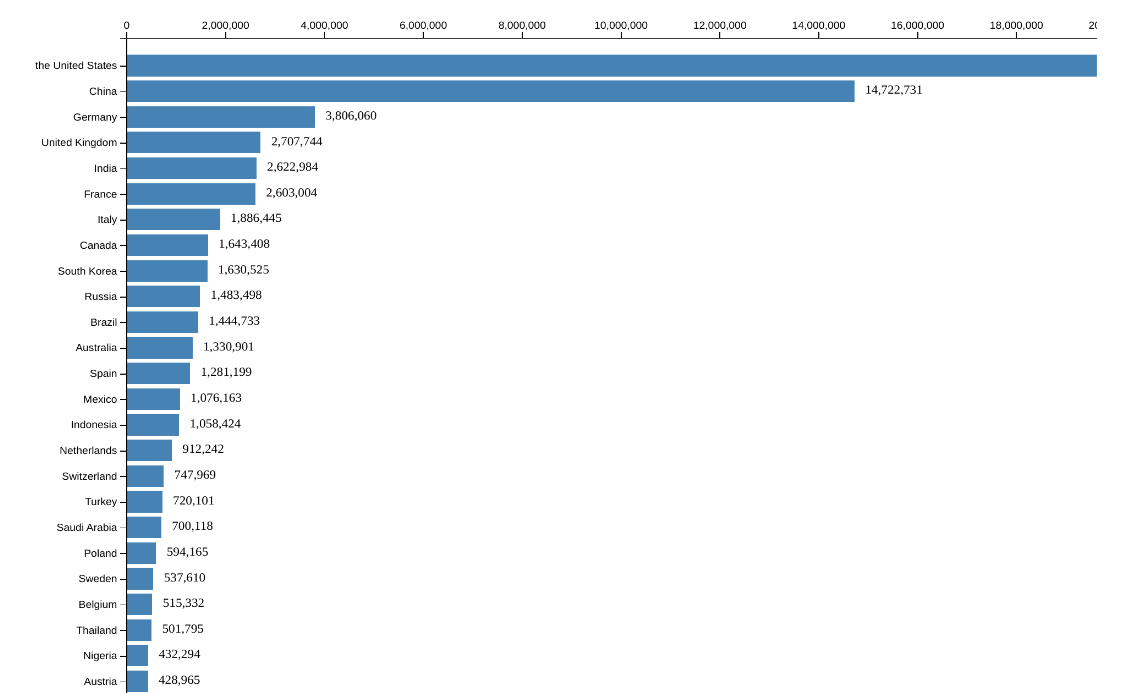
\includegraphics[width=.9\linewidth]{./charts/gdp_per_country.png}
\end{center}

\begin{itemize}
\item A horizontal bar chart was chosen here to show the GDP per country
\begin{itemize}
\item Note: The image was cut off slightly when saving to pdf/screenshot, please load and view the actual webpage instead.
\end{itemize}
\item Visual encoding here includes:
\begin{itemize}
\item Length - Denoting the total amount of GDP for that country in year 2020
\end{itemize}
\end{itemize}
\subsection{Global Distribution of GDP}
\label{sec:org727fb53}

\begin{center}
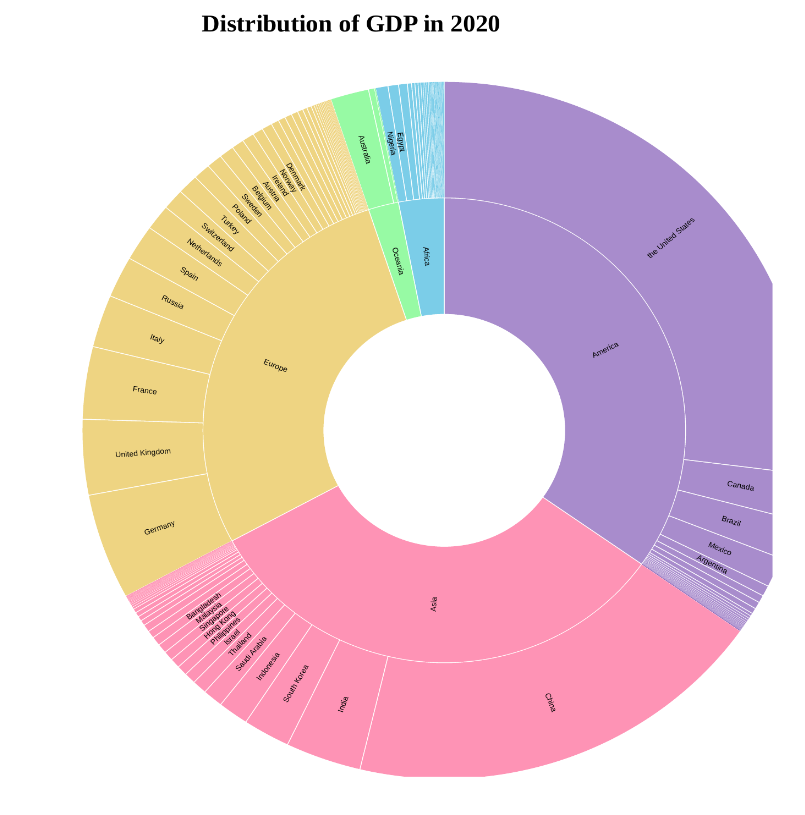
\includegraphics[width=.9\linewidth]{./charts/gdp_sunburst.png}
\end{center}

\begin{itemize}
\item A sunburst chart was chosen to show both the distribution/percentages of GDP across the countries as well as across regions.
\begin{itemize}
\item Note: The image was cut off slightly when saving to pdf/screenshot, please load and view the actual webpage instead.
\end{itemize}
\item Visual encoding here includes:
\begin{itemize}
\item Length - Denoting the percentage of total GDP globally that the country makes up
\item Color - Differentiating the regions
\end{itemize}
\item Insights
\begin{itemize}
\item From the chart, it is evident how United States and China alone makes up for approximately a third of the world's GDP.
\end{itemize}
\end{itemize}
\subsection{Regional Distribution of GDP (in millions) in 2020}
\label{sec:org03fb628}
\begin{center}
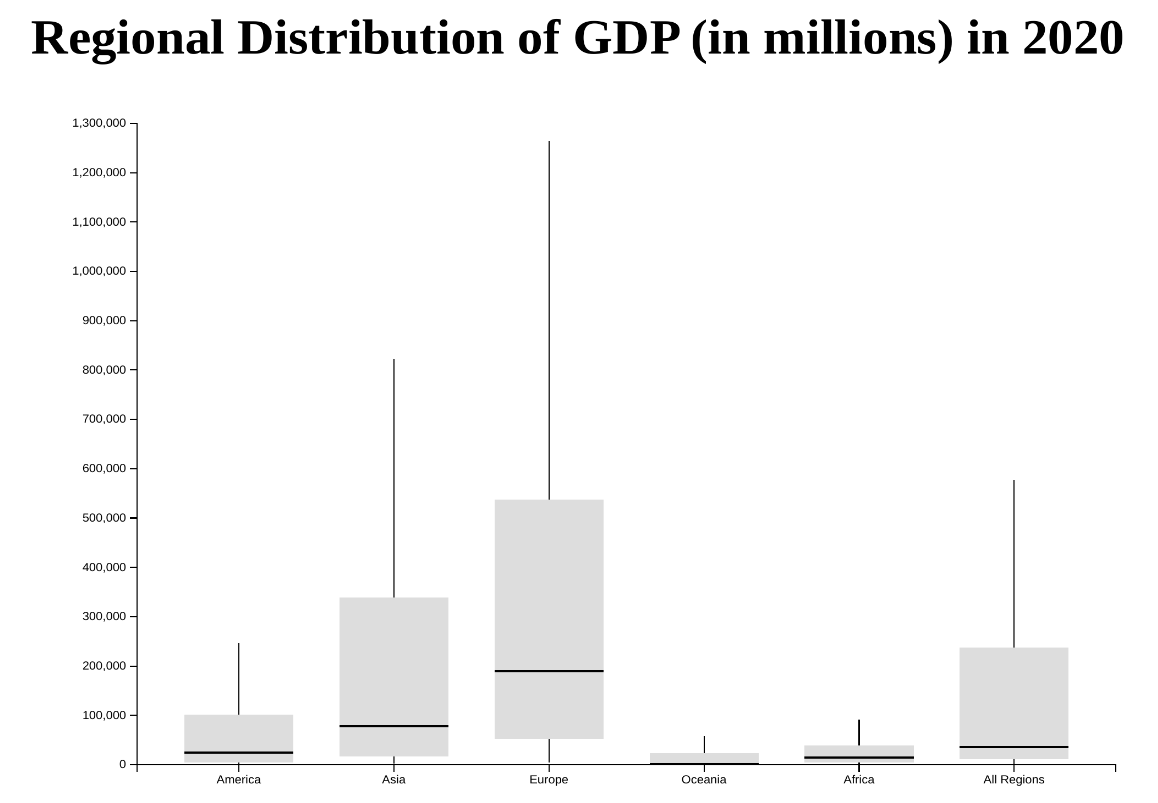
\includegraphics[width=.9\linewidth]{./charts/gdp_boxplot.png}
\end{center}
\begin{itemize}
\item A boxplot was chosen here to show the distribution/stats of GDP spread across various regions.
\item Visual encoding here includes:
\begin{itemize}
\item Position - Denoting the amount of GDP
\end{itemize}
\item Insights
\begin{itemize}
\item Of particular interest is that outliers aside, the region ``America'' does not actually do very well in spite of United States ranking first in terms of total GDP.
\item It is also quite fascinating to see that Europe fared the best when looking at median and the interquartile range.
\end{itemize}
\end{itemize}
\end{document}
